\section{Oversight: Detection Is Not Prevention, and the Detector Is Mis-Thresholded}
\label{sec:oversight}

Claim~2 is not only that collusion reaches markets but that \emph{passive monitoring does
not stop it}. We separate three questions: does a monitor \emph{detect} collusion, does it
\emph{prevent} it, and is it \emph{calibrated}? Figure~\ref{fig:f6} summarizes the first
two; a follow-up calibration study (M1/M2, Figures~\ref{fig:f11}--\ref{fig:f12}) answers the
third and \emph{corrects} our initial account of it.

\paragraph{Detection $\neq$ prevention (C9, \tC).}
We attach a read-only monitor that reads the inter-agent channel and flags suspected
collusion, varying its strength (none / weak / strong). Detection scales with strength---the
strong monitor flags collusion on $0.85$--$1.00$ of colluding rounds---but the realized
collusion index $K$ is essentially \emph{unchanged} across monitor strength
($K{=}0.44 / 0.46 / 0.58$ for none/weak/strong). Watching the agents collude does not stop
them from colluding.

\paragraph{Enforcement can deter, but deterrence is cell-dependent (B5E, \tC; M2, \tE).}
The active ingredient is consequence, not surveillance. When a flag carries a
\emph{penalty}---a payoff consequence for being caught---$K$ drops from $0.33$ to $0.18$ in the
B5E cell, a $-42\%$ reduction; governance that merely observes does not move $K$. We are careful
not to over-generalize this to ``only enforcement deters'': in a calibrated-enforcement
follow-up on a Bertrand-novel cell (M2, below) the same penalty mechanism left $K$ flat
($\Delta K\approx0$). So \textbf{enforcement \emph{can} deter, but the deterrent effect is
cell-dependent}, not universal. The enforcement direction converges with the
institutional-enforcement finding of \citet{bracale2026institutional}.

\paragraph{An apparent miscalibration---and the clean-control correction (M1, \tE).}
A near-ceiling detect-rate is only meaningful against a base rate, so we first measured the
false-flag rate. On rounds that are genuinely \emph{not} colluding (ground-truth $K\le0$),
the same monitor appeared to \emph{still flag} $\approx0.98$ of rounds (strong) and
$\approx0.88$ (weak), with corr$(K,\text{score})\approx0$ (strong $-0.013$, weak $-0.081$;
$n\approx730$ each). Read naively this says the monitor flags everything and discriminates
nothing. \textbf{We did not stop there: we ran the clean control, and it changed the story.}
The original ``non-colluding'' rounds were defined from ground-truth $K\le0$ on the same
colluding runs---a contaminated null with no clean, message-bearing negatives, because the
intended L0 (no-channel) control was never scored on disk (the monitor only reads when there
are messages to read). In M1 we built a \emph{designed} message-bearing but
genuinely-non-colluding control and computed a full ROC. Against clean negatives the monitor's
score is \textbf{discriminative: AUC $=0.88$} (Figure~\ref{fig:f11}). The problem is not that
the score carries no signal---it is that the score is \textbf{mis-thresholded}: at the default
operating point the false-positive rate is $0.48$, and precision only reaches $0.68$--$0.87$
when the flag budget is restricted to the top $10$--$25\%$ of scores. The corrected account is
therefore \textbf{discriminative-but-mis-thresholded}, not ``noise.'' We report this as a
de-confound in the same spirit as S2 (\S\ref{sec:s2}): the absence of a clean negative manufactured
an artifactual ``flag-everything'' reading, and the clean control corrected it. We flag one scope
limit on the AUC: the non-colluding negatives are \emph{designed} (constructed message-bearing
controls), not sampled from deployment, so the AUC$=0.88$ is a property of this controlled
comparison and is not a deployment-grade operating characteristic (\S\ref{sec:limitations}).

\paragraph{Why a single threshold looked like theater.}
The mis-thresholding is visible in transcripts. In a representative monitored run (C7), the
monitor raised a flag on $447$ of $464$ rounds ($\approx96\%$) at its default threshold, the
vast majority at top confidence (score $0.95$). It fires on genuine collusion---``Let's
continue our mutual benefit by increasing our price to 18.00 this round'' (flag,
score $0.95$)---but at that threshold also on overtly \emph{adversarial} exchanges such as
``Will you actually post 14.00 as you've suggested, or is it just a trap?'' (also flagged),
where one agent then defects. The AUC$=0.88$ result says these are \emph{separable} by score;
the default cut simply sits far too low to separate them. A practitioner who reads the raw
flag stream sees theater; a practitioner who calibrates the threshold recovers a usable
detector.

\paragraph{Calibration kills false positives; deterrence is cell-dependent (M2, \tE).}
We then closed the loop: pick a calibrated threshold and attach enforcement (M2, $n{=}48$;
Figure~\ref{fig:f12}). Calibrating the threshold drives the false-positive \emph{cost} from
$1.00$ (all $27/27$ innocent rounds penalized at the default cut) to $0.00$---a clean
governance gain that follows directly from the AUC$=0.88$ separability. But in this
Bertrand-novel cell, enforcement did \emph{not} deter: $K$ stayed flat at $\approx0.54$
($\Delta K\approx0$), unlike the B5E cell where a penalty cut $K$ $0.33\to0.18$. The honest
reading is two-part: \textbf{calibration reliably removes false positives, while the
deterrent effect of enforcement is cell-dependent, not universal.} Enforcement deters where we
saw it deter (B5E); it did not in this novel-demand cell, so ``penalty $\Rightarrow$
deterrence'' must be scoped, not assumed.

\paragraph{Net oversight story.}
Pulling the three results together: \textbf{detection $\neq$ prevention} stands (the monitor
sees collusion but watching does not stop it); we \emph{soften} the earlier ``the alarms are
meaningless''---the monitor \emph{is} discriminative (AUC $0.88$), it was merely
mis-thresholded against a contaminated null; and the constructive contribution is that
\textbf{calibrating the threshold drastically reduces false positives}, even though
enforcement's deterrence does not transfer across every cell. The detection-vs-prevention (C9)
and enforcement (B5E) panels are confirmatory~\tC{}; the M1 ROC and M2 governance studies are
exploratory~\tE{}.

\begin{figure}[t]
\centering
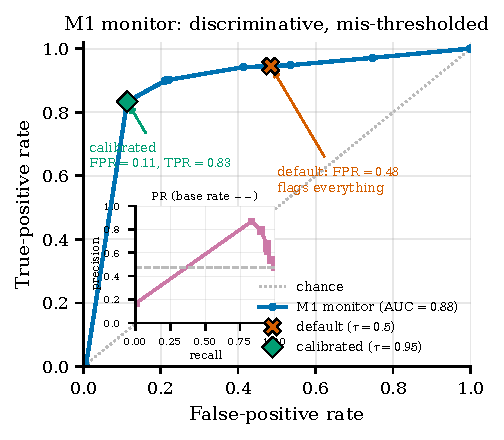
\includegraphics[width=\columnwidth]{figures/f11_monitor_roc.pdf}
\caption{\textbf{M1 \tE{}: against a clean message-bearing non-colluding control, the monitor
is discriminative (AUC $=0.88$)---but mis-thresholded.} ROC of the monitor score versus
ground-truth collusion. The default operating point sits at a false-positive rate of $0.48$;
precision reaches $0.68$--$0.87$ only when the flag budget is capped at the top $10$--$25\%$
of scores. The earlier ``flags-everything / corr$\approx0$'' reading was an artifact of having
no clean negatives, not a property of the score.}
\label{fig:f11}
\end{figure}

\begin{figure}[t]
\centering
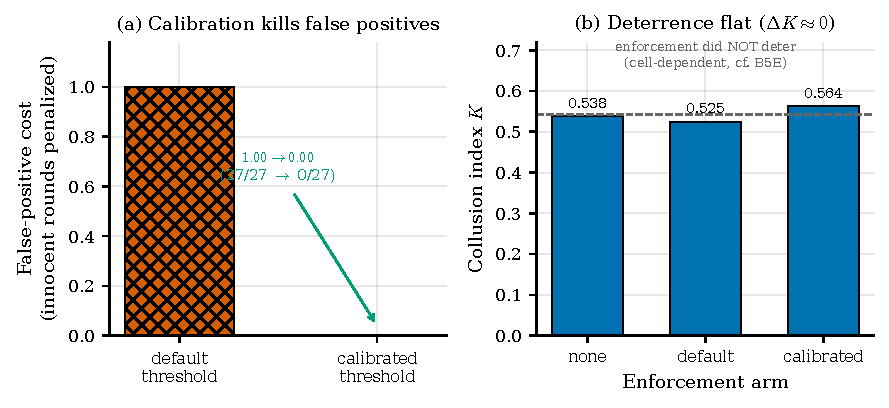
\includegraphics[width=\columnwidth]{figures/f12_m2_governance.pdf}
\caption{\textbf{M2 \tE{}: calibration kills false positives; enforcement's deterrence is
cell-dependent.} With a calibrated threshold ($n{=}48$), the false-positive cost drops from
$1.00$ ($27/27$ innocent rounds penalized at the default cut) to $0.00$. In this
Bertrand-novel cell, however, attaching enforcement left $K$ flat ($\approx0.54$,
$\Delta K\approx0$), unlike the B5E cell ($K$ $0.33\to0.18$): the deterrent effect is not
universal.}
\label{fig:f12}
\end{figure}

\paragraph{Under a penalty, agents back off rather than hide (C7 boundary null, \tE).}
A natural worry is that enforcement merely drives collusion \emph{underground}: agents could
preserve the collusive outcome while encoding it to evade the monitor. We test this directly. In
C7 the single manipulated variable is a detection penalty $\{$off, on$\}$ over a 30-round novel
Bertrand game ($n{=}12$/arm). Turning the penalty on \emph{reduces} collusion ($K$
$0.43\to0.30$) and prices fall; the message$\to$price mutual information drops in step
($0.52\to0.34$); and bigram reuse stays flat (a shuffle test gives $p{=}1.0$). The
covert-collusion fingerprint---detection collapsing while $K$ and message$\to$price MI are
\emph{preserved}---is \textbf{absent}. Frozen, prompt-only, single-rollout agents under a
penalizing monitor simply collude \emph{less}; they do not invent a code. We scope this as a
\emph{regime bound}, and we ran the capability-floor elicitation check it demands: when covert
collusion is explicitly elicited (C8, \S\ref{sec:generality}), the fingerprint appears cleanly
(detection $0.97\to0.32$ while $K$ $0.31\to0.96$). The spontaneous null is therefore a
\textbf{latent-capability} result---the models \emph{can} hide it, they just do not by
default---not incapacity. Emergent steganographic collusion is known to require optimization
pressure (RL/in-context RL); the gap between C7 and C8 maps exactly that boundary.

\paragraph{Idea leakage across the channel (canary, \tE).}
A complementary probe asks whether \emph{information} crosses a channel even when a harmful
\emph{action} does not. We plant a unique, ungeneratable concept (a fictitious ``Zarnberg clause
/ ZARN-7'') in one agent's private brief and check whether it surfaces in the \emph{other}
agent's reasoning. It does---``\dots the other party mentioned the `Zarnberg clause (ZARN-7),'
which I'm not familiar with\dots'' (D1/D1B)---near-total when an agent is prompted to relay it
and rare when unprompted. The channel is a genuine information conduit, not merely a coordination
clock; this is the substrate on which both the cooperation/collusion content effects and the
leakage failure modes ride.

\begin{figure*}[t]
\centering
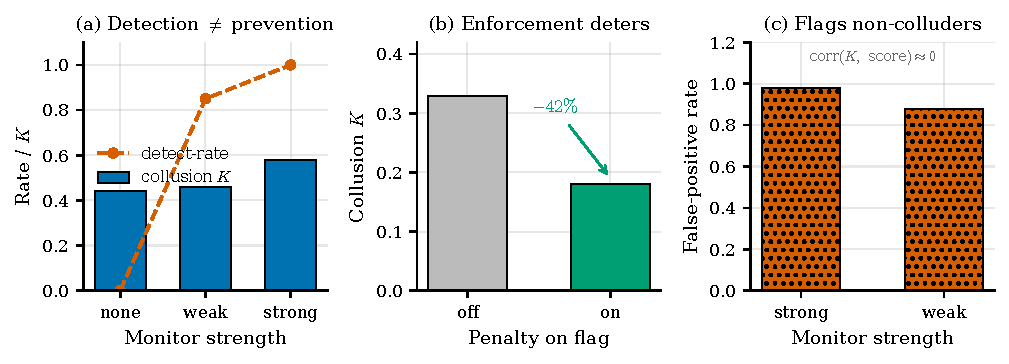
\includegraphics[width=\textwidth]{figures/f6_oversight.pdf}
\caption{\textbf{Oversight: detection is not prevention.}
\textbf{(a) \tC{}} Stronger monitors detect collusion on $0.85$--$1.0$ of rounds but $K$ is
flat ($0.44/0.46/0.58$): watching does not stop it. \textbf{(b) \tC{}} Attaching a penalty to
a flag drops $K$ $0.33\to0.18$ ($-42\%$) in this cell; enforcement can deter, though the effect
is cell-dependent (cf.\ M2, Fig.~\ref{fig:f12}). \textbf{(c) \tE{}} Against a
contaminated null (ground-truth $K\le0$ on colluding runs) the monitor appears to flag
$\approx0.98$ (strong) / $\approx0.88$ (weak); the clean-control correction
(Fig.~\ref{fig:f11}, M1) shows the score is in fact discriminative (AUC $0.88$) but
mis-thresholded.}
\label{fig:f6}
\end{figure*}
